\section{Proposed Method}
\label{sec:method}

In this section, we describe the details of our methods, including PLNPR and UltraNPR. Given a noisy and large-scale OM brain image, PLNPR aims to obtain a robust and accurate reconstruction of neurons from local noisy image blocks, while UltraNPR aims to reconstruct complete neuronal populations from a large-scale image more efficiently.
%In the reminder of this section, we first introduce the PLNPR algorithm, then we detail the UltraNPR algorithm.
%The pipeline of our methods is shown in Fig.~\ref{fig:framework}.
%In the reminder of this section, we first introduce the PLNPR, a unsupervised progressive learning algorithm which can significantly improve neuronal population reconstruction performance without using manual annotations. Then we detail the UltraNPR algorithm for reconstructing neuronal population from a ultra-scale 3D mouse brain slice.


\subsection{PLNPR for Robust Neuronal Population Reconstruction}
%\subsection{Unsupervised Progressive Learning for Neuronal Population Reconstruction}
\label{sec:PLNPR}

To reconstruct neuronal populations from noisy OM images, our PLNPR algorithm consists of three key components: a segmentation network, an image enhancement module and a neuron tracing module, as shown in Fig.~\ref{fig:framework}. 
%
The segmentation network is designed to extract neuron voxels from noisy and complex backgrounds.
%\de{To reconstruct neurons from noisy OM images, our PLNPR method consists of three key components: a segmentation network, image enhancement module, and a neuron tracing module, as shown in Fig.~\ref{fig:framework}. The segmentation network is designed to first extract neuron voxels from noisy and complex background.}
%
Then, instead of using a binary mask of the segmented voxels, we employ a probability map predicted by the network and integrate it with the raw image intensities in order to simultaneously preserve the global neuron structure and local neurite details.
After that, the neuron tracing module is applied to reconstruct neurons from the enhanced image block.
%However, existing segmentation networks are trained with strong supervision, and dense voxel-wise annotations are required. Instead of acquiring annotations with huge human efforts, 
We progressively train the segmentation network with the reconstructed neurons inferred from conventional tracing methods as labels, and improve the reconstruction results from better neuron segmentation.
%\de{Instead of acquiring manual annotations with huge efforts, we progressively train the segmentation network with the reconstructed neurons as labels using conventional neuron tracing methods,}
Based on the iterative learning process, the powerful DNNs and tracing methods mutually complement and promote each other to gradually improve the neuron reconstruction performance.


\subsubsection{Progressive Learning without Annotations}
\label{sec:PL}

%In order to learn discriminative and representative features for extracting neuron voxels, we train the segmentation network with the reconstructed neurons as the 
In order to train the segmentation network to learn discriminative features for extracting neuron voxels, we use the reconstructed neurons to provide pseudo labels.
%
In each iteration of segmentation and reconstruction, we apply the NGPST~\cite{Quan2015} as the neuron tracing module to reconstruct neurons from image blocks. This module can be replaced by any tracing method that does not require manual annotations for training.
%\de{we utilize the NGPST~\cite{Quan2015} to reconstruct a neuronal population in the OM image. The neuron tracing module can be replaced by any tracing method that does not require voxel-wise annotations for training.}
It takes an image block $\mathbf{B}$ in size of $S\times H \times W$ as input and reconstructs a neuronal population with separated neurons.
%The intensity $\mathbf{I}(x)$ of a voxel $x$ belongs to $[0,1]$.
From the reconstruction results, we produce a binary mask $\mathbf{M}$ indicating foreground by $\mathbf{M}(x)=1$ and background by $\mathbf{M}(x)=0$ for a voxel $ x $.



Given $N$ image blocks, we train our segmentation network using the neuron masks $\{\mathbf{M}_i, i=1,\cdots,N\}$ generated from the neuron tracing module.
Details of the network architecture and training strategy are described in Sec.~\ref{sec:network}.
The output of the neuron segmentation network is a 3D probability map $\mathbf{P}$, which is computed by a voxel-wise softmax activation function. $\mathbf{P}(x)\in [0,1]$ indicating the probability of a voxel $x$ to be a neuron part.
Then, by fusing the predicted probability map with the raw intensities, the raw block is further enhanced in order to preserve both local signals and global structures simultaneously. Details are introduced in Sec.~\ref{sec:enhancement}.
When the enhanced block is used as input to the neuron tracing module, more complete neuronal populations can be reconstructed.
%\de{Then the raw image is further enhanced by fusing the predicted probability map with the raw intensities in order to preserve both global structures and local signals simultaneously.Details are introduced in Sec.~\ref{sec:enhancement}. %here the weak neuron signals will be enhanced, as show in Fig. \ref{fig:framework}. By feeding the enhanced image to the neuron tracing module, more complete neuronal populations can be reconstructed.}

\subsubsection{DNN for 3D Neuron Segmentation}
\label{sec:network}

Considering the size, morphology and intensity of neurons vary significantly, extracting neuron voxels from image blocks is not a trivial problem.
In recent years, many 3D DNNs, such as 3D U-Net~\cite{Cicek2016}, 3D DSN~\cite{Dou2017} and DenseVoxNet~\cite{Yu2017} have demonstrated an outstanding capability in various biological and biomedical image segmentation tasks.
Therefore, we take advantage of 3D segmentation networks to extract more representative features to meet the challenges of neuron segmentation.
In this work, the 3D DSN is extended as our neuron segmentation network to balance the performance and computation burden.
%\de{Since neurons vary significantly in size, morphology, and intensity, we take the advantage of 3D segmentation networks to extract more representative features to meet the challenges of neuron segmentation from 3D OM images. The network can be any end-to-end trainable 3D segmentation network, such as 3D U-Net~\cite{Cicek2016}, 3D DSN~\cite{Dou2017} and DenseVoxNet~\cite{Yu2017}. In this paper, we extend the 3D DSN as our neuron segmentation network to balance the performance and computation burden.} 
%In addition, to further validate the robustness and effectiveness of our algorithm, we also test several different networks in our framework and the results are introduced in Sec.~\ref{sec:experiments}.


The 3D DSN network consists of convolutional layers, pooling layers and deconvolutional layers, all in 3D fashion. The convolutional layers and pooling layers act as feature extractor, while the deconvolutional layers followed by softmax layer aim to up-sample the feature maps to the same size as the input. To further boost the information flow within the network, two more branches are employed to connect the shallower layers to the output layer. These connections strengthen the gradient propagation, stabilize the learning process, and further taps the potential of the limited training data to learn more discriminative features. %Please refer to~\cite{Dou2017} for more details.


Although 3D DSN has achieved excellent performance for 3D organ segmentation~\cite{Dou2017}, it is still prone to overfitting in our case due to the limited training data.
%\de{Although DSN has demonstrated its excellent performance in volumetric medical image segmentation, it is still prone to overfitting in our case due to limited training data.}
One common solution to this problem is to combine the predictions of several DNN models at the test time. However, this approach will greatly reduce the efficiency of the system.
Instead of training several models simultaneously, we employ a more efficient alternative solution for network training, which is known as Dropout~\cite{Srivastava2014}.
This technique can significantly reduce node interactions and help the network to learn more robust features that better generalize to new data.
In our network, the dropout with a rate of $0.5$ is applied to every convolutional layer.
%In our network, the dropout layer is implemented following each convolutional layer with the dropout rate of $0.5$.
%\de{We employ the dropout technique for our network training and the dropout layer is implemented following each convolutional layer with the dropout rate of $0.5$.}


Another challenge of training 3D DNN is the memory limitation because the 3D feature images are huge with respect to the input size. Therefore, for each input image block, we crop a group of cubes in size of $160\times 160\times 160$ with $30\%$ overlaps, and set batch size to 1 during training. Correspondingly, at the test time, we stitch these overlapped probability cubes together using average blending to get a probability map in the same size with the input block.


In addition, the volume of neuron (foreground) voxels is usually much smaller than that of background in an OM image.
To cope with this imbalance problem, a data balancing technique is introduced for network training.
%This highly imbalance problem could suppress the performance of the segmentation network. To cope with this problem, a data balancing technique is introduced for network training.
Specifically, when computing the training loss, we only consider the neuron voxels and a certain portion of background voxels, which is randomly selected as non-neuron samples.
The number of non-neuron voxels used for training is set as $10$ times that of neuron voxels.
%\de{Moreover, the volume of non-neuron voxels is typically much larger than that of neurons in images. This data imbalance could suppress the performance of the neuron segmentation network. We use a data balancing technique to address the problem. Specifically, for each cube, we randomly select a certain portion of background voxels as non-neuron samples, while the rest background voxels are not included in the loss computation. The number of background voxels for training is set as $10$ times that of neuron voxels.}

Last but not least, to have the same physical resolution with the lateral dimension in OM image blocks, voxels along the axial dimension are interpolated after the imaging process. However, it makes the image quality along different dimensions inhomogeneous. In order to alleviate the impact of this problem on network training, a random transposition process is employed for each cube as data augmentation.
%\de{Last but not the least, voxel intensities along the axial dimension in OM images are interpolated to the same resolution with the lateral dimension after the imaging process. Due to the inhomogeneity of imaging quality along different dimensions, a random transposition process of each cube is employed as data augmentation for training.}

%To train the networks, we use the stochastic gradient descent algorithm with the Adam update rule as the stochastic optimization strategy and a categorical cross-entropy loss function. We use a decaying learning rate starting from 1?−4 and gradually decreased to 1?−7 on the last epoch. We use an early stopping policy by monitoring validation performance and picked the best model with the highest accuracy on the validation set.

\subsubsection{Image Enhancement}
\label{sec:enhancement}

After finishing the network training, we use the trained model to predict the probability cube for each input cube.
Then, by stitching all probability cubes together, we can obtain the probability map $\mathbf{P}$ for the entire raw image block $ \mathbf{B} $.
Each element in $\mathbf{P}$ indicates the probability that the corresponding voxel in $ \mathbf{B} $ belongs to the neuron.
To utilize the probability map, one natural way is to reconstruct neurons directly from it.
However, since the pseudo labels is not as accurate as manual annotations, the performance of the segmentation network is limited. As a result, the predicted probability map may not cover all neurons and some local details may be lost, especially for the first few iterations.
In our method, an enhanced representation is generated by fusing the probability map and original raw image block, in order to keep detailed structures and suppress noise signals effectively.
Specifically, a new probability map $\widetilde{\mathbf{P}} $ is first constructed by linearly mapping the value range of $ \mathbf{P}\in [0,1] $ to the value range $[\mathbf{B}_{min}, \mathbf{B}_{max}]$ of $\mathbf{B}$.
%\de{By using the trained segmentation network, a probability cube of the corresponding input cube is predicted. Then all probability cubes are stitched together to obtain a probability map $\mathbf{P}$ for the entire image stack. Each element of $\mathbf{P}$ indicates the probability of the corresponding voxel as a neuron, known as foreground probability. A natural way to use the probability map is to apply the tracing algorithm directly on it to reconstruct neurons. However, due to the limited performance of the DNN network that is trained with pseudo labels, the probability map may not cover all neurons and lose some signal details compared to the raw image $ \mathbf{I}$, especially at the first few iterations. In our approach, we fuse the original raw image and the probability map together to get an enhanced representation, in order to suppress noise signals and keep detailed structures effectively. Specifically, we construct a new probability map $\widetilde{\mathbf{P}} $ by linearly mapping the  value range of $ \mathbf{P}\in [0,1] $ to the value range $[\mathbf{I}_{min}, \mathbf{I}_{max}]$ of the raw image $\mathbf{I}$.}
\begin{equation}
\widetilde{\mathbf{P}}(x) = (\mathbf{B}_{max}-\mathbf{B}_{min})\mathbf{P}(x).
\end{equation}


Then, base on the raw image block $\mathbf{B}$ and the probability map $\widetilde{\mathbf{P}}$, an enhanced image block $\mathbf{E}$ is computed as
\begin{equation}
\mathbf{E}(x) = \alpha\widetilde{\mathbf{P}}(x) + (1-\alpha)\mathbf{B}(x),
\label{equ: enhance}
\end{equation}
where $\alpha\in [0,1]$ is a weight to control the contributions of voxel $ x $ in the original intensity and the probability map. By feeding the enhanced blocks to the neuron tracing module, neuronal populations can be reconstructed more completely.
%\de{Then we use a straightforward way to compute an enhanced image $\mathbf{A}$ from the probability map $\widetilde{\mathbf{P}}$ and the raw image $\mathbf{I}$ as where $\alpha$ is a weight to control the contributions of voxel $ x $ in the probability map and the original intensity. When the enhanced images are used as input to the neuron tracing module, morce complete neuronal populations can be reconstructed.}


With more reliable reconstruction results for supervision, the segmentation network could be further trained to learn more discriminative and representative features for producing probability maps, which in turn benefits the tracing module to reconstruct neurons in the next iteration.
%Our system progressively improves the neuron reconstruction performance by combining conventional tracing methods and DNNs without any manual annotations.
\begin{figure}[t]
	\centering
	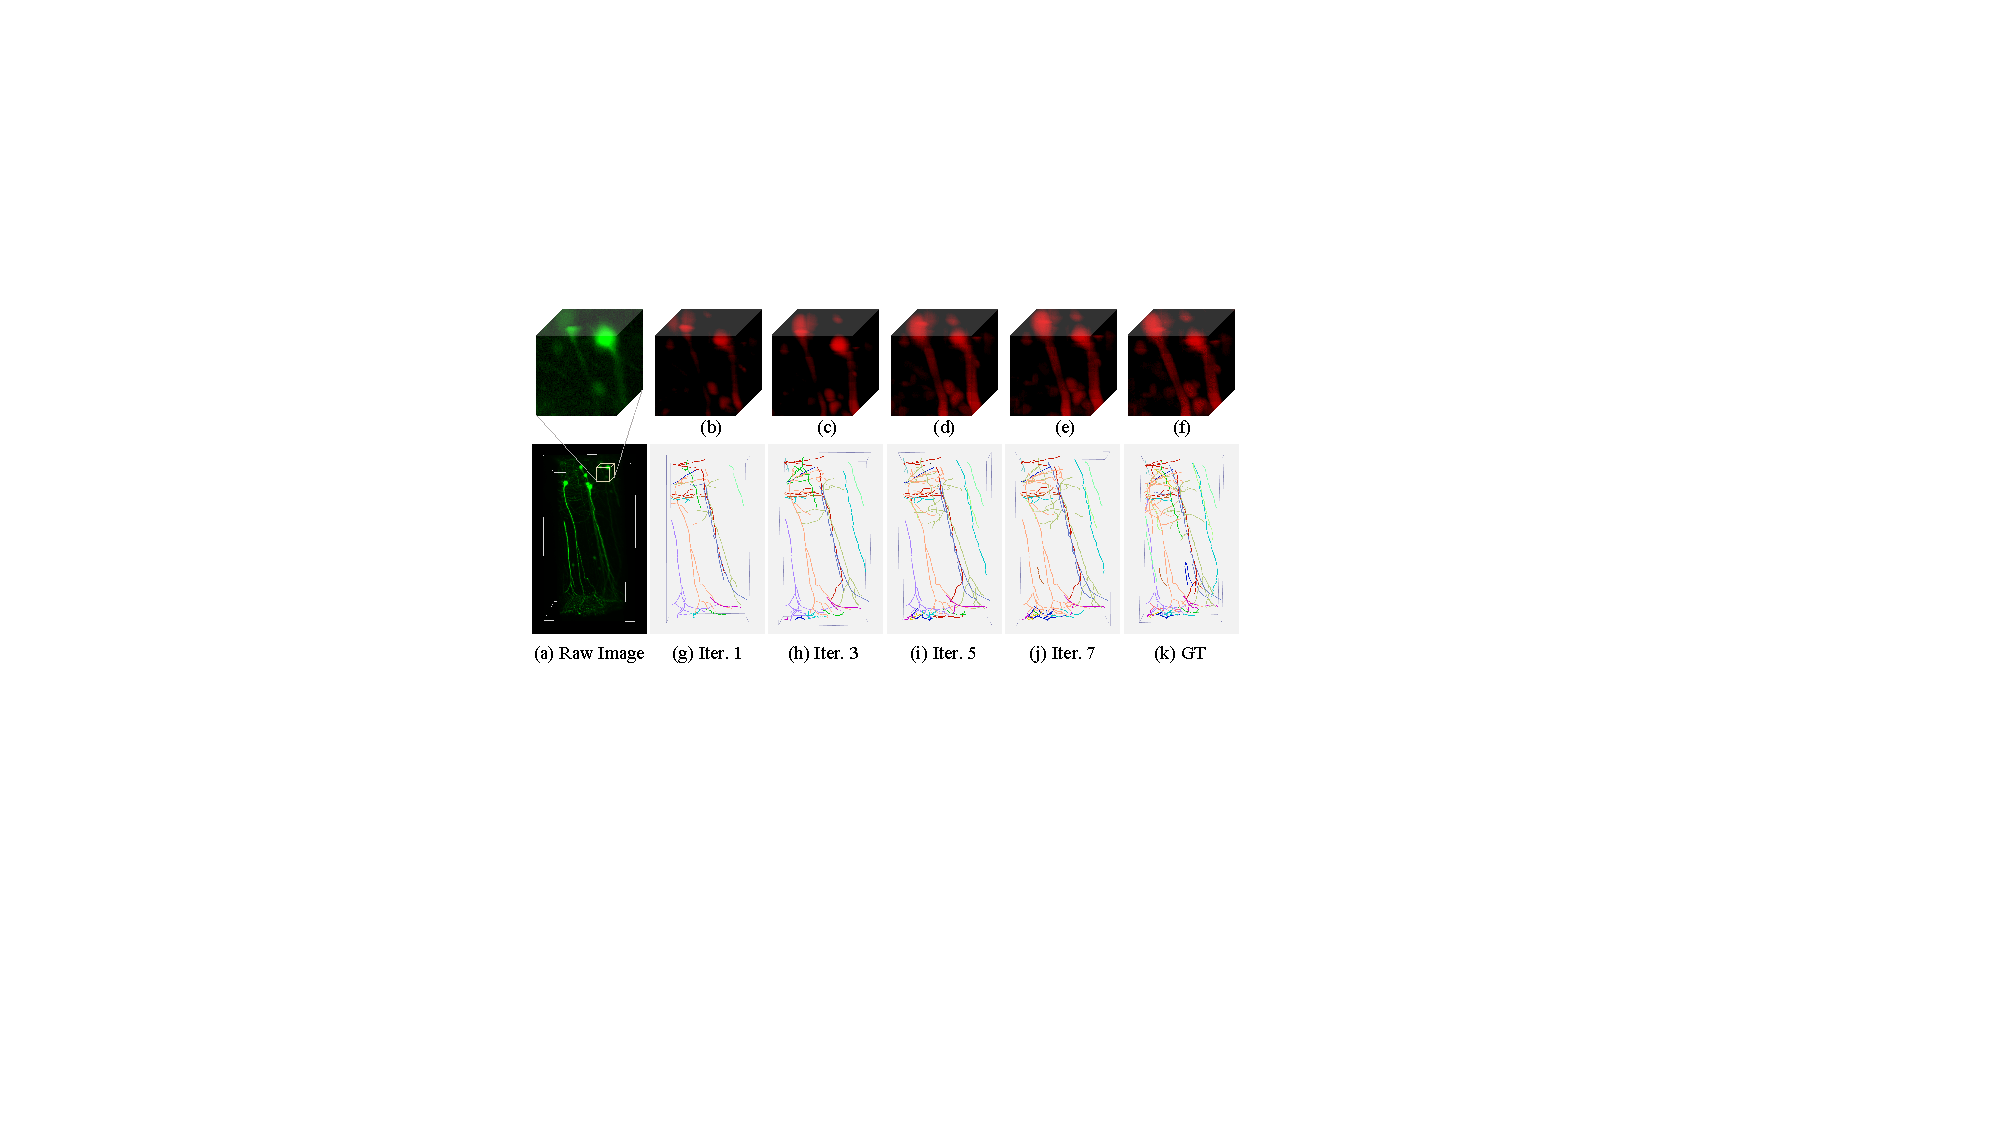
\includegraphics[width=1\columnwidth]{./Illustrations/ngps.pdf}
	\caption{
		Our progressive learning technique gradually improves the segmentation network to extract neuron signals from (a) raw image which has noises and low contrast. (b)(c)(d)(e) The probability maps generated by the segmentation network at different iterations. (f) Combing the probability map and the raw intensity, the enhanced block preserves both global trajectory and local details. (g)(h)(i)(j) More and more complete and accurate reconstruction of the neuronal populations can be obtained with more iterations. (k) The manually labeled neurons are shown for comparison. Separated neurons are shown in different colors.}
	\label{fig:ngps}
\end{figure}
%
As shown in Fig.~\ref{fig:ngps}(a), due to the noises and low contrast in the raw image block, the intensity of neuron voxels is inhomogeneous, which makes some neurons subtle.
%At first, by feeding the raw image to the conventional method~\cite{Quan2015}, a neuronal population can be reconstructed. However, compared to the ground truth (GT) shown in Fig.~\ref{fig:ngps}(k), the reconstructed neuronal population is incomplete and many neurites are missing, as Fig.~\ref{fig:ngps}(g) shows.
At first, comparing with the ground truth (GT) shown in Fig.~\ref{fig:ngps}(k), the neurons reconstructed from the raw image block are incomplete and many neurites are missing, as shown in Fig.~\ref{fig:ngps}(g).
Then, by utilizing the pseudo labels derived from imperfect reconstruction, the segmentation network can be trained to learn features for global trajectories. Fig.~\ref{fig:ngps}(b) shows the predicted probability map, which demonstrates the enhanced trajectories.
With more iterations of neuron reconstruction and network training, more distinctive and long-range trajectory features can be progressively captured by the network, as shown in Fig.~\ref{fig:ngps}(c)(d)(e).
By combining the original image intensities with the predicted probability map, both local signal details and global trajectories are well preserved in the enhanced block, as Fig.~\ref{fig:ngps}(f) shows.
%In order to preserve global trajectories and local signal details well, we combine the original image intensities with the predicted probability map. The enhanced image is shown in Fig.~\ref{fig:ngps}(f).
Iteration by iteration, the completeness and accuracy of neuron reconstruction are increasingly improved, as shown in Fig.~\ref{fig:ngps}(h)(i)(j).
%the neuronal populations are reconstructed more and more completely and accurately, as shown in Fig.~\ref{fig:ngps}(h)(i)(j).
%\de{As shown in Fig.~\ref{fig:ngps}(a), neurites are subtle because of the low contrast and noises in the raw image. At the beginning, the reconstructed neurons are incomplete and many neurites are missing, as Fig.~\ref{fig:ngps}(g) shows, compared to the ground truth (GT) shown in Fig.~\ref{fig:ngps}(k). Then trained by the pseudo labels derived from non-perfect reconstruction, the segmentation network is able to learn features for global trajectories, and the predicted probability maps demonstrate the enhanced trajectories, as Fig.~\ref{fig:ngps}(b) shows. With more iterations of network training and neuron reconstruction, our segmentation network captures more distinctive and long-range trajectory features progressively, as shown in Fig.~\ref{fig:ngps}(c)(d)(e). By combining the probability map with the raw image intensities, both global trajectories and local signal details are well preserved. Fig.~\ref{fig:ngps}(f) shows the enhanced image. Iteration by iteration, the reconstruction of neuronal populations becomes more and more complete and accurate, as shown in Fig.~\ref{fig:ngps}(h)(i)(j).}









\subsection{Large-scale Neuronal Population Reconstruction}
\label{sec:UltraNPR}

\begin{figure*}[th]
	\centering
	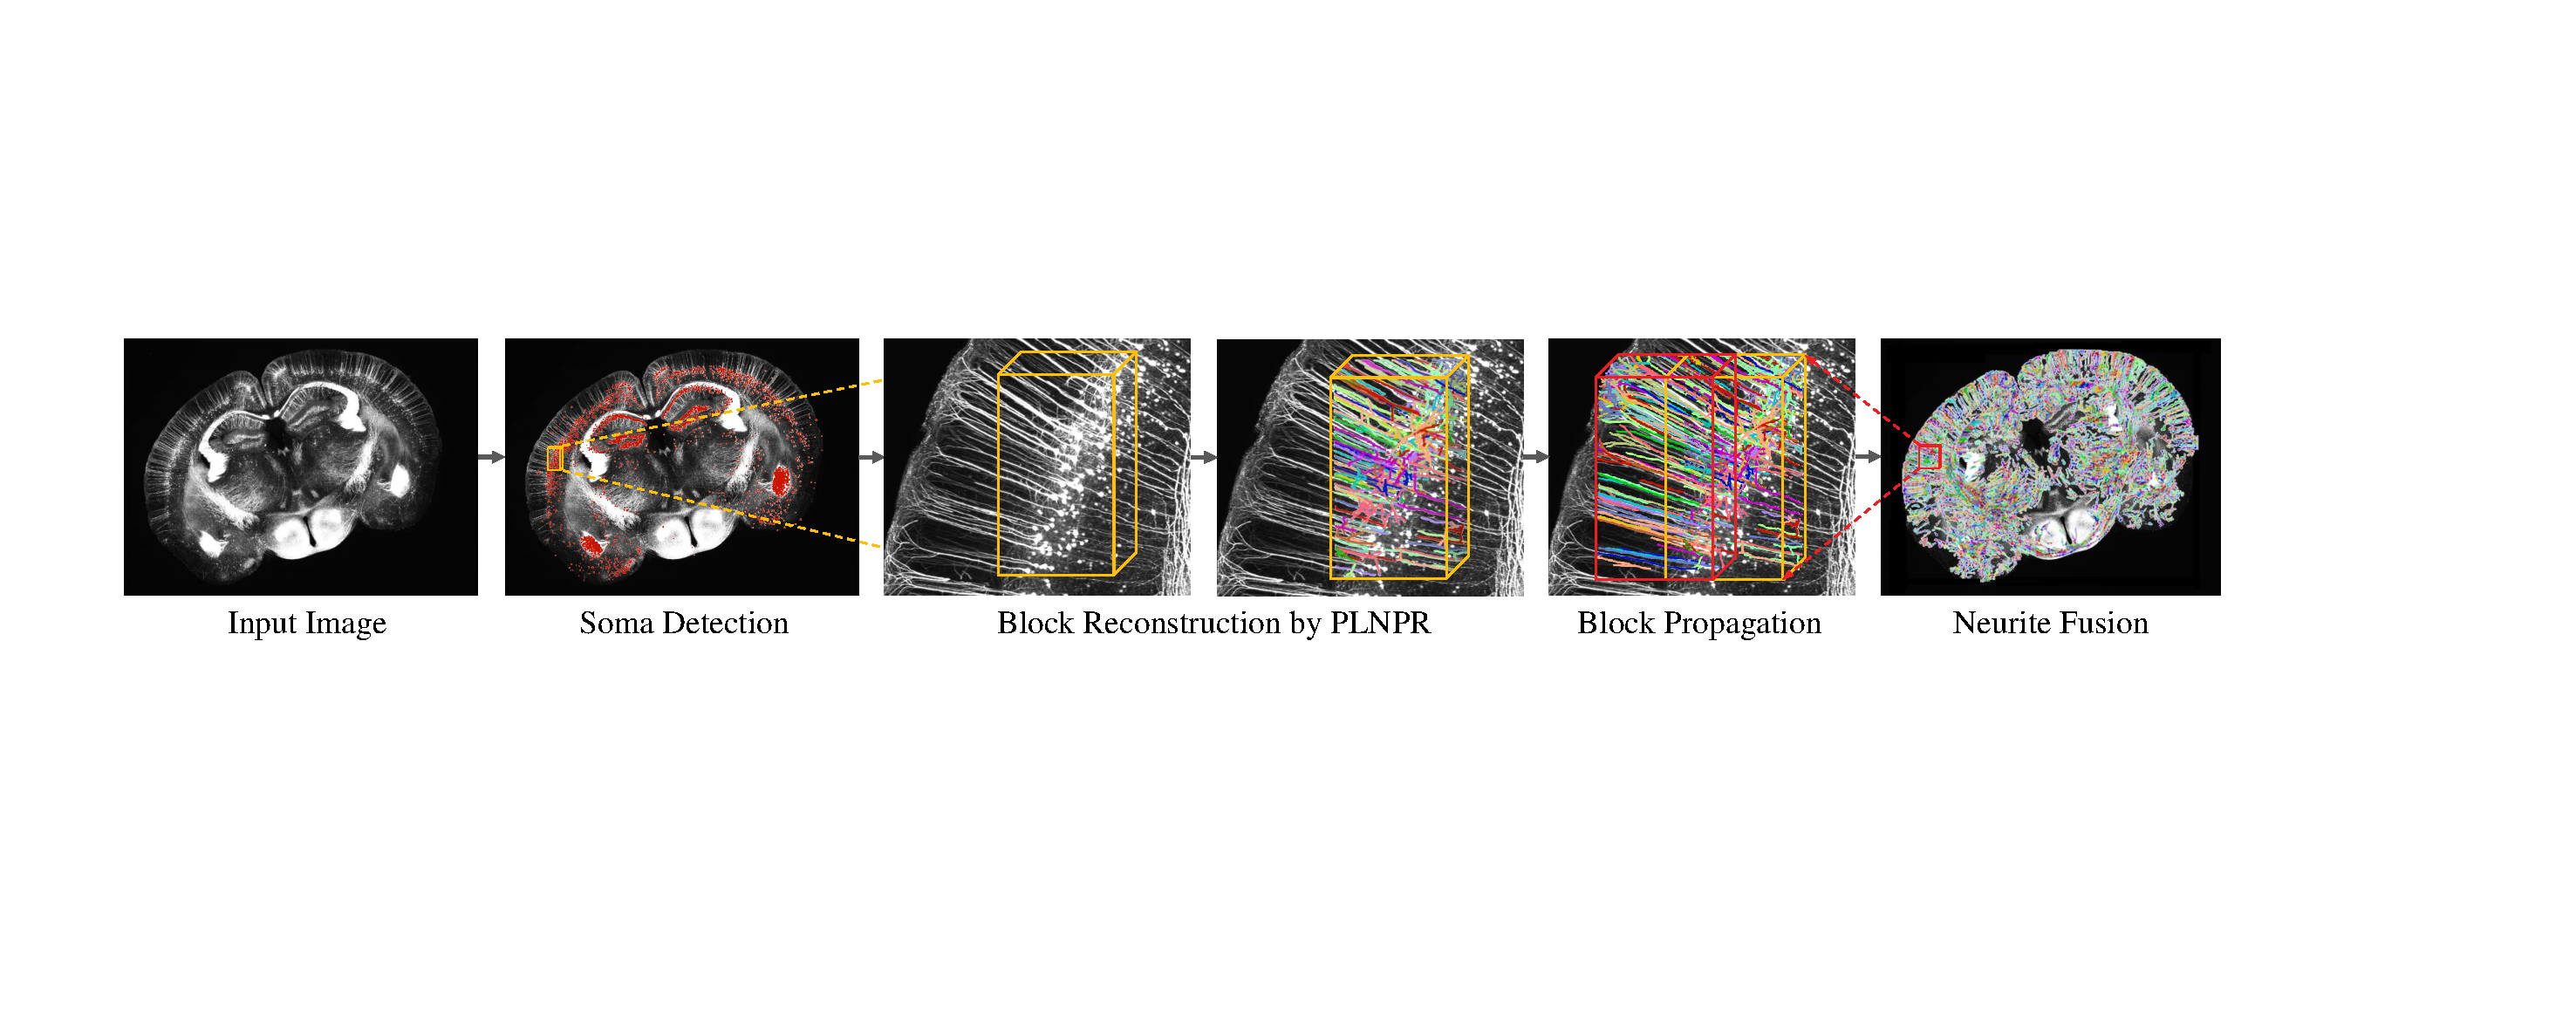
\includegraphics[width=1\textwidth]{./Illustrations/framework_ultranpr.PNG}
	\caption{Diagram of our UltraNPR algorithm for neuronal population reconstruction in a large-scale brain slice.}
	\label{fig:ultra_framework}
\end{figure*}

To reconstruct neuronal populations from a large-scale 3D image, our UltraNPR consist of four key components: a soma detection module, a local reconstruction module, a block search module, and a neurites fusion module, as shown is~\ref{fig:ultra_framework}.
At first,  the large-scale image is divided into overlapped 3D blocks of the same size. 
The soma detection module is used to detect somas from the large-scale image.
The local reconstruction module is based on our PLNPR algorithm to reconstruction neurons from low-quality image blocks. 
Then, to reconstruct the large-scale image block by block,  we repeatedly use the block search module to determine what the next block needs to be reconstructed. 
After that, the neurites fusion module is applied to obtain a complete and continuous reconstruction from adjacent blocks.

\subsubsection{Initial Soma Detection}
\label{sec:soma}

To detect somas from the large-scale image efficiently, we apply soma detection algorithm~\cite{Quan2013} on each block separately.
However, due to the overlap between blocks, somas in the overlapped area would be detected repeatedly.
To tackle this over-detection error, we map all detected somas from local blocks to the coordinate system of the original image and merge the overlapped somas by averaging their position and radius.
The soma detection results from the large-scale image are visualized in Fig.~{4} of the supplementary file.
These somas are also used to define the initial blocks for neuron reconstruction in the next step.


%\subsubsection{Large-scale Neuronal Population Reconstruction}
\subsubsection{Block Search Policy and Local Reconstruction}
\label{sec:trace}

The neuronal population reconstruction $\mathbf{R}$ in a large-scale image can be modeled as the joint performance of the reconstruction in each block $\mathbf{B}_i$.
Given an image $\mathbf{I}$, performing a local tracing method $T$ to reconstruct neuronal populations block by block can be formulated as follows
\begin{equation}
\mathbf{R} = T(\mathbf{I}) = T(\mathbf{B}_1, \mathbf{B}_2,\cdots,\mathbf{B}_N).
\end{equation}

As somas are where signals from the dendrites are joined and pass on, the blocks containing somas are the most probable locations to start the tracing.
Therefore, the initial blocks that contain somas are firstly reconstructed by our PLNPR method.
The reconstruction produced by PLNPR is represented by a series of neuronal compartments. The neuronal compartments which are close to the block boundary typically indicate the continuity of the structure of neurons. We call these compartments as terminal tips and use them as the potential continuous signals for searching the next blocks to grow the neuronal structure from each initial block.
%
Then, neurons in the next blocks are reconstructed by PLNPR based on the terminal tips provided by adjacent blocks that have already been reconstructed.
By iteratively searching the next blocks, UltraNPR can reconstruct neuronal populations more and more completely.

%
In addition, due to the dense distribution of neurons in the brain image, fragmented neurites belonging to different neurons could be in the same block, which means some blocks may be repeatedly reconstructed starting from different initial blocks.
To more efficiently explore the structure of neuronal populations, for each searching direction of an initial block, the iterative searching process will be terminated when the next block contains somas or no new terminal tips could be detected.


\subsubsection{Neurites Fusion from Adjacent Blocks}
Since neurons would be split into fragmented neurites when dividing the raw image into blocks, neurites from adjacent blocks need to be maximally connected, and the connection should be as continuous and smooth as possible.
As fragment neurites in the overlapping area may belong to different neurons, we first match them by comparing the overlapping region between every two neurites from adjacent blocks.
Then, the matched neurites are assembled to get a continuous and smooth reconstruction. 

However, simply assembling them would cause over-tracing error and topological discrepancy, as shown in Fig.~\ref{fig:overlap_discrepancy}.
The over-tracing error is caused by the overlap between blocks when the respective neurites from these blocks are assembled.
The topological discrepancy is mainly caused by the lack of context information for tracing methods, which makes the reconstruction near the block boundary often inaccurate and unreliable.
But this region is inside the adjacent block due to the overlap between them, which means substantial context information of this region can be provided to the tracing methods and leads to a better reconstruction.
Therefore, when assembling two matched neurites from adjacent blocks, we only consider neuronal compartments which are not near the boundary of the corresponding block. 

\begin{figure}[t]
	\centering
	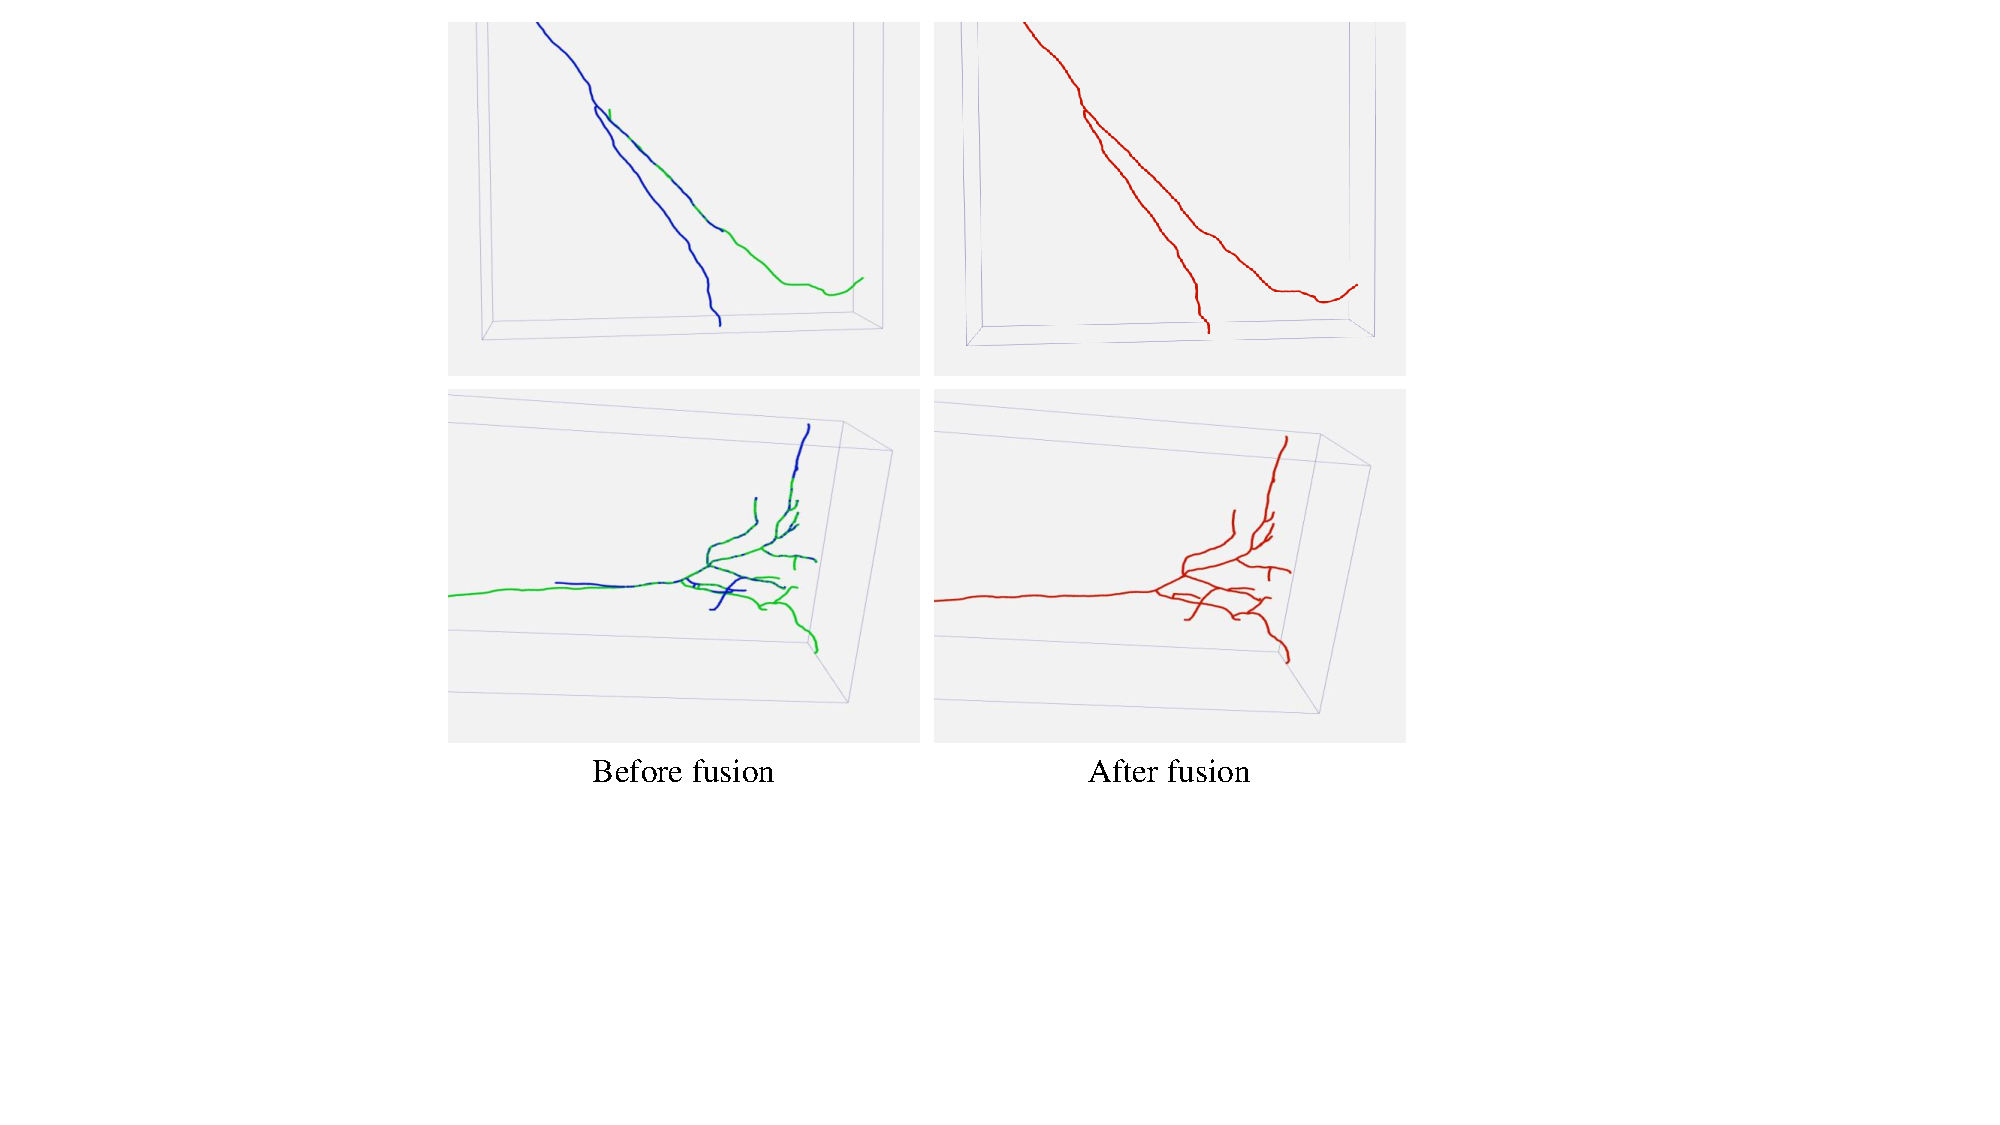
\includegraphics[width=1\columnwidth]{./Illustrations/neuorns_fusion2.pdf}
	\caption{Two examples of correcting the over-tracing and topological discrepancy errors by our fusion algorithm. These reconstructions are shown in skeleton mode for better visualization.}
	\label{fig:overlap_discrepancy}
\end{figure}

\begin{figure}[t]
	\centering
	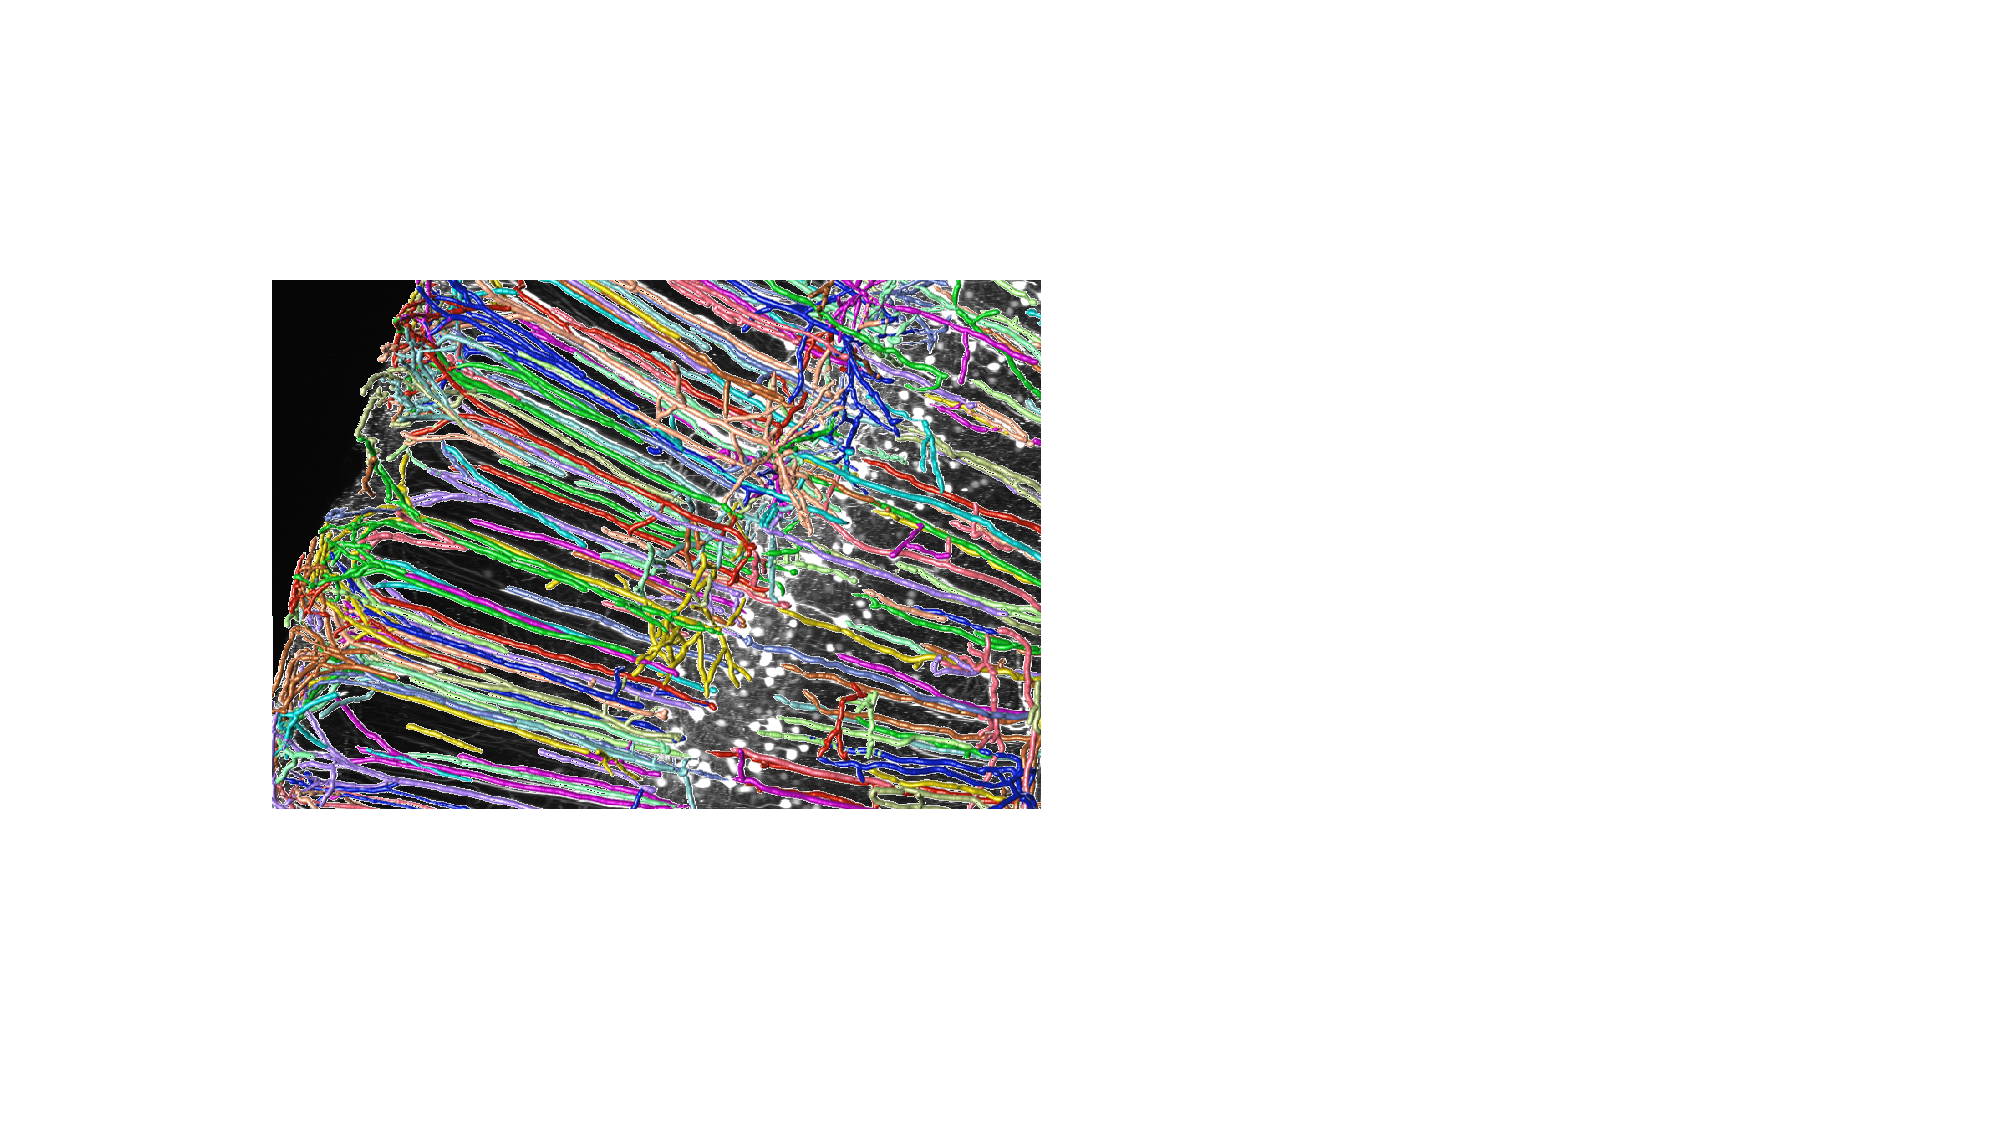
\includegraphics[width=1\columnwidth]{./Illustrations/trace_four_blocks2.pdf}
	\caption{One example of reconstructing neuronal populations from four adjacent blocks using our method. We can observe that, the fragmented neurites from adjacent blocks are assembled continuously and smoothly.}
	\label{fig:reconstruct_blocks}
\end{figure}

Based on the above observations, a fusion algorithm is designed to assemble the matched neurites.
Concretely, we first calculate the length of two neurites and select the longer one as the reference neurite. Here, we use $\mathcal{N_A}$ to denote the reference neurite, and $\mathcal{N_B}$ to denote another neurite.
Then, for each branch $\mathcal{H_B}$ in neurite $\mathcal{N_B}$, we search in neurite $\mathcal{N_A}$ to see if there is a branch $\mathcal{H_A}$ that overlaps with it.
%
If yes, three steps will be performed to assemble the two branches together.
Firstly, we remove the neuronal compartments in branch $\mathcal{H_A}$ and branch $\mathcal{H_B}$ that near the boundary of the corresponding block, and all branches that are connected to the removed compartments will also be removed. Here, this distance is set to be $70$ voxels.
Secondly, for each neuronal compartment in branch $\mathcal{H_B}$, if there are compartments of branch $\mathcal{H_A}$ around it, it will be removed; otherwise, it is considered to be valid. The searching radius is empirically set to be $10$ voxels.
%Thirdly, by searching the nearest compartment in branch $\mathcal{H_A}$, the modified branch $\mathcal{H_B}$ is connected to $\mathcal{H_A}$.
Thirdly, the first compartment in the modified branch $\mathcal{H_B}$ is connected to $\mathcal{H_A}$ by searching the nearest compartment in branch $\mathcal{H_A}$. 
%In this way, branches in neurite $\mathcal{N_B}$ can be merged with the neurite $\mathcal{N_A}$.
When all branches $\mathcal{H_B}$ overlapping with the neurite $\mathcal{N_A}$ are processed, we can obtain the assembled neurite $\mathcal{N_{AB}}$.
If there are remaining branches $\mathcal{H_B}$ which are not overlapped with neurite $\mathcal{N_A}$, the $\mathcal{N_{AB}}$ will be updated by assembling the remaining branches $\mathcal{H_B}$.
%After all branch $\mathcal{H_B}$ overlapping with neurite $\mathcal{N_A}$ are assembled with neurite $\mathcal{N_A}$, the remaining branches in neurite $\mathcal{N_B}$ will be connected to the assembled neurite $\mathcal{N_{AB}}$ by searching the neatest compartment in $\mathcal{N_{AB}}$.
%In this way, neurite $\mathcal{N_B}$ and neurite $\mathcal{N_A}$ can be merged.



Fig.~\ref{fig:overlap_discrepancy} shows two examples of correcting the over-tracing and topological discrepancy errors by our algorithm.
As shown in Fig.~\ref{fig:reconstruct_blocks}, the neuronal population from four adjacent blocks are successfully reconstructed from the noisy images by our UltraNPR method and the fragment neurites in adjacent blocks are assembled continuously and smoothly.
%It can be seen that the neuronal population is successfully reconstructed from the noisy images and the fragment neurites in adjacent blocks are assembled continuously and smoothly.
%The overall ``UltraNPR"" algorithm can be found in Algorithm~\ref{alg:reconstruction}.


\begin{figure}[t]
	\centering
	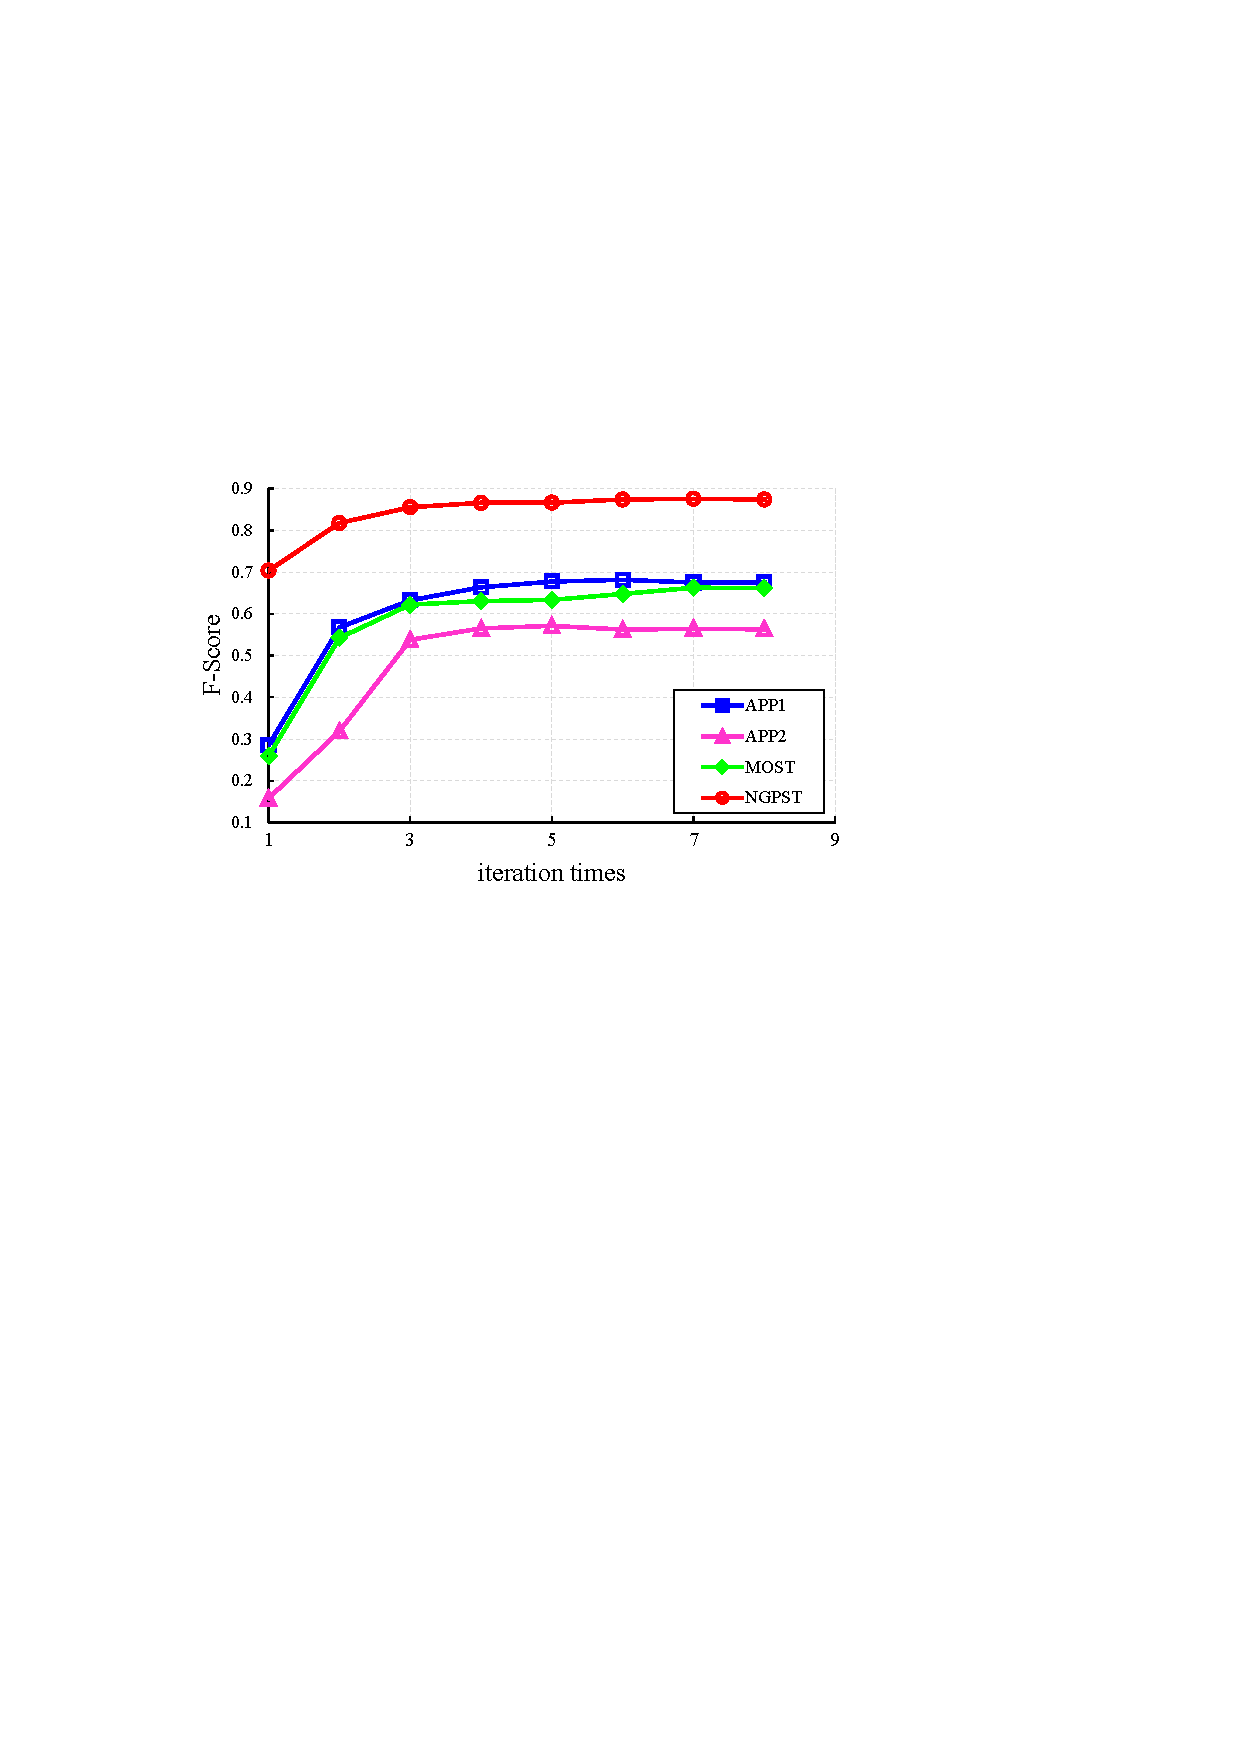
\includegraphics[width=\columnwidth]{./Illustrations/trace_iterations_fscore8.pdf}
	\caption{F-Score of neuron reconstruction using four neuron tracing methods APP1~\cite{Peng2011} and its variant APP2~\cite{Xiao2013}, MOST\cite{Wu2014} and NGPST~\cite{Quan2015} on the VISoR-40 test dataset at eight iterations. For each of the four neuron tracing methods, our approach progressively improves their reconstruction results.} 
	%Plots of other metrics are available in the supplementary materials.}
	\label{fig:fscore_iterations}
\end{figure}


\delete{
\subsection{Large-scale Neuronal Population Reconstruction}
\label{sec:UltraNPR}

\begin{figure*}[th]
	\centering
	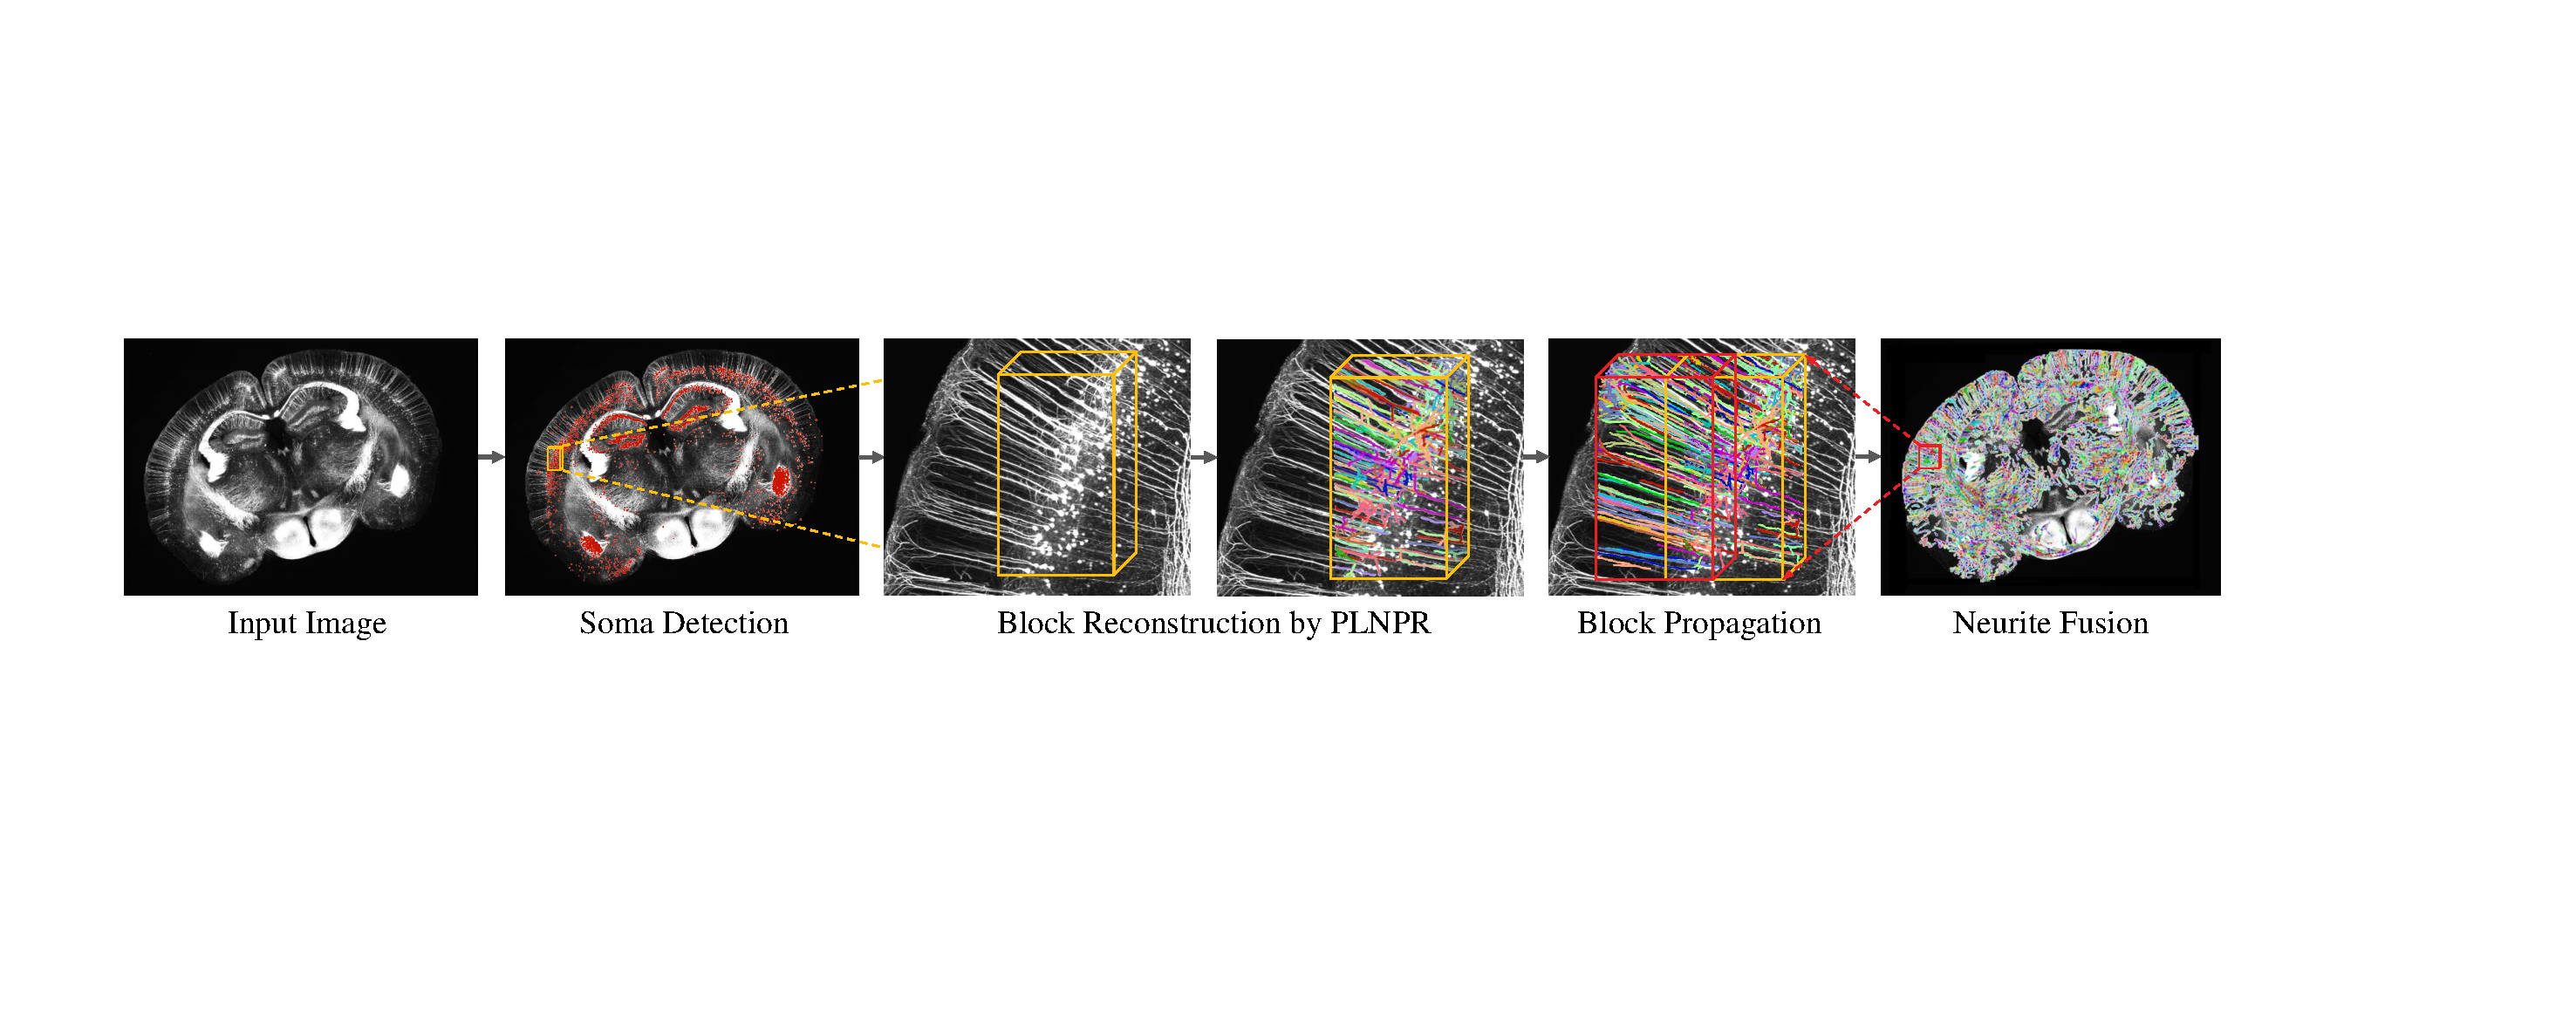
\includegraphics[width=1\textwidth]{./Illustrations/framework_ultranpr.pdf}
	\caption{Diagram of our UltraNPR algorithm for neuronal population reconstruction in a large-scale brain slice.}
	\label{fig:ultra_framework}
\end{figure*}

To reconstruct neuronal populations from a large-scale image, our UltraNPR consist of three key components: a local reconstruction module, a block search module, and a neurites fusion module, as shown is~\ref{fig:ultra_framework}.
The local reconstruction module is based on our PLNPR algorithm to reconstruction neurons from low-quality image blocks. Then, to reconstruct the large-scale image block by block,  we repeatedly use the block search module to determine what the next block needs to be reconstructed. After that, the neurites fusion module is applied to obtain a complete and continuous reconstruction from adjacent blocks.

The proposed PLNPR successfully traces neurons from low-quality and megabyte-sized local image blocks. However, for a large-scale high resolution OM brain image, the image size is formidably large in a terabyte scale, which is far beyond the processing capability of existing tracing methods, especially for the memory cost.
%including our PLNPR algorithm.
%in dimension of $25397\times 18516\times 869$.
%The image used for studying large-scale neuron reconstruction is shown in Fig.~\ref{fig:brain}, a mouse brain slice with image resolution of $25397\times 18516\times 869$. 
%These terabyte-sized images are far beyond the processing capability of existing tracing methods, including our PLNPR algorithm.
%The image size is formidably large in a terabyte scale.

To reconstruct neuronal populations from a large-scale image, the basic idea of our UltraNPR algorithm is to reconstruct neurons block by block.
The image used in this work is shown in Fig.~\ref{fig:brain}, a mouse brain slice with image resolution of $25397\times 18516\times 869$.
%
As shown in Fig~\ref{fig:ultra_framework}, our UltraNPR algorithm consists of three key components.
%: soma detection, 
%
First of all, the large-scale image is divided into 3D blocks of the same size. 
Considering the raw image size and the computational efficiency, the block size is set to be $1120\times 2048\times 869$. 
In addition, we introduce $300$ voxels overlap between adjacent blocks to avoid false continuation and increase the robustness of the reconstruction.
%avoid detection errors and tracing errors in soma detection and neuron reconstruction separately.
To obtain a complete and continuous reconstruction from blocks, UltraNPR consists of two steps: soma detection and neuronal population reconstruction.

\subsubsection{Initial Soma Detection}
\label{sec:soma}

To detect somas from the large-scale image efficiently, we apply soma detection algorithm~\cite{Quan2013} on each block separately.
However, due to the overlap between blocks, somas in the overlapped area would be detected repeatedly.
%To remove these duplicate detection results, we first map all somas to a unified spatial coordinate system of the brain slice.
To tackle this over-detection error, we map all detected somas from local blocks to the coordinate system of the original image and merge the overlapped somas by averaging their position and radius.
%the position and radius of the merged soma are the average of the position and radius of the overlapped somas, respectively.
%Fig.~\ref{fig:detected_soma} shows the detected somas of the brain image.
The soma detection results from the large-scale image are visualized in Fig.~{4} of the supplementary file.
These somas are also used to define the initial blocks for neuron reconstruction in the next step.


%\subsubsection{Large-scale Neuronal Population Reconstruction}
\subsubsection{Block Search Policy and Local Reconstruction}
\label{sec:trace}

The neuronal population reconstruction $\mathbf{R}$ in a large-scale brain image can be modeled as the joint performance of the reconstruction in each block $\mathbf{B}$.
Given an image $\mathbf{I}$, performing a tracing method $T$ to reconstruct neuronal populations block by block can be formulated as follows
\begin{equation}
\mathbf{R} = T(\mathbf{I}) = T(\mathbf{B}_1, \mathbf{B}_2,\cdots,\mathbf{B}_N).
\end{equation}
%
Since neurons would be split into fragmented neurites when dividing raw image into blocks, neurites from adjacent blocks need to be maximally connected, and the connection should be as continuous and smooth as possible.
We use an intuitive approach to solve this problem, by repetitively searching the next block according to the neurons in already-reconstructed blocks. This process can be factorized as follows
\begin{equation}
\begin{aligned}
&\mathbf{R}_1 =  T(\mathbf{B}_1), \\
&\mathbf{R}_2 =  T(\mathbf{B}_2 | \mathbf{R}_1), \\
&\mathbf{R}_3 =  T(\mathbf{B}_3 | \mathbf{R}_1, \mathbf{R}_2),\\
&\cdots\\
&\mathbf{R} =  T(\mathbf{B}_N | \mathbf{R}_1, \mathbf{R}_2, \cdots, \mathbf{R}_{N-1}).\\
\end{aligned}
\end{equation}

As somas are where signals from the dendrites are joined and pass on, the blocks containing somas are the most probable locations to start the tracing.
UltraNPR uses the PLNPR method to reconstruct neurons from the blocks that contain somas at first.
%Typically, the neuronal compartments closed to the block boundary indicate the continuity of the structure of neurons. Therefore, we detect the terminal tips from these boundary compartments.
The neuron reconstruction produced by PLNPR is represented by a series of neuronal compartments. The neuronal compartments which are close to the block boundary typically indicate the continuity of the structure of neurons. We call these compartments as terminal tips and use them as the potential continuous signals for searching the next blocks to grow the neuronal structure from each initial block.
%To grow the neuronal structure from each initial block, terminal tips are used as the potential continuous signals for searching the next blocks.
%Typically, the neuronal compartments closed to the block boundary indicate the continuity of the structure of neurons. Therefore, we detect the terminal tips from these boundary compartments.
Then, neurons in the next blocks are reconstructed by PLNPR based on the terminal tips provided by adjacent blocks that have already been reconstructed.
By iteratively searching the next blocks, UltraNPR can reconstruct neuronal populations more and more completely.
%
However, due to the dense distribution of neurons in the brain image, fragmented neurites belonging to different neurons could be in the same block, which means some blocks may be repeatedly reconstructed starting from different initial blocks.
To more efficiently explore the structure of neuronal populations, for each searching direction of an initial block, the iterative searching process will be terminated when the next block contains somas or no new terminal tips could be detected.



%%%%%%%%%%%%%%%%%%%%%%%%%%%%%%%%%%%%%%%%%%%%%%
\subsubsection{Neurites Fusion from Adjacent Blocks}
After reconstructing neurons from all blocks, UltraNPR analyzes the reconstructed neurites to obtain a complete neuronal population reconstruction.
%between adjacent blocks, and applies the following fusion algorithm to assemble them.
%
Since fragment neurites in the overlapping area may belong to different neurons, we first match them by comparing the overlapping region between every two neurites from adjacent blocks.
%Since fragment neurites of different neurons may be in the overlapping area between two adjacent blocks, we first map these neurites by comparing the overlapping region between neurites.
Then, the matched neurites are assembled to get a continuous and smooth reconstruction. 


However, simply assembling them would cause over-tracing error and topological discrepancy, as shown in Fig.~\ref{fig:overlap_discrepancy}.
%
The over-tracing error is caused by the overlap between blocks when the respective neurites from these blocks are assembled.
%so that the overlapped neuronal compartments need to be assembled during the fusion process.
The topological discrepancy is mainly caused by the lack of context information for tracing methods, which makes the reconstruction near the block boundary often inaccurate and unreliable.
At the same time, this region is inside the adjacent block due to the overlap between them, which means substantial context information of this region can be provided to the tracing methods and leads to a better reconstruction.
Therefore, when assembling two matched neurites from adjacent blocks, we only consider neuronal compartments which are not near the boundary of the corresponding block. 
%Here, this distance is empirically set to be $70$ voxels.
%``neurite A"``neurite B"

\begin{figure}[t]
	\centering
	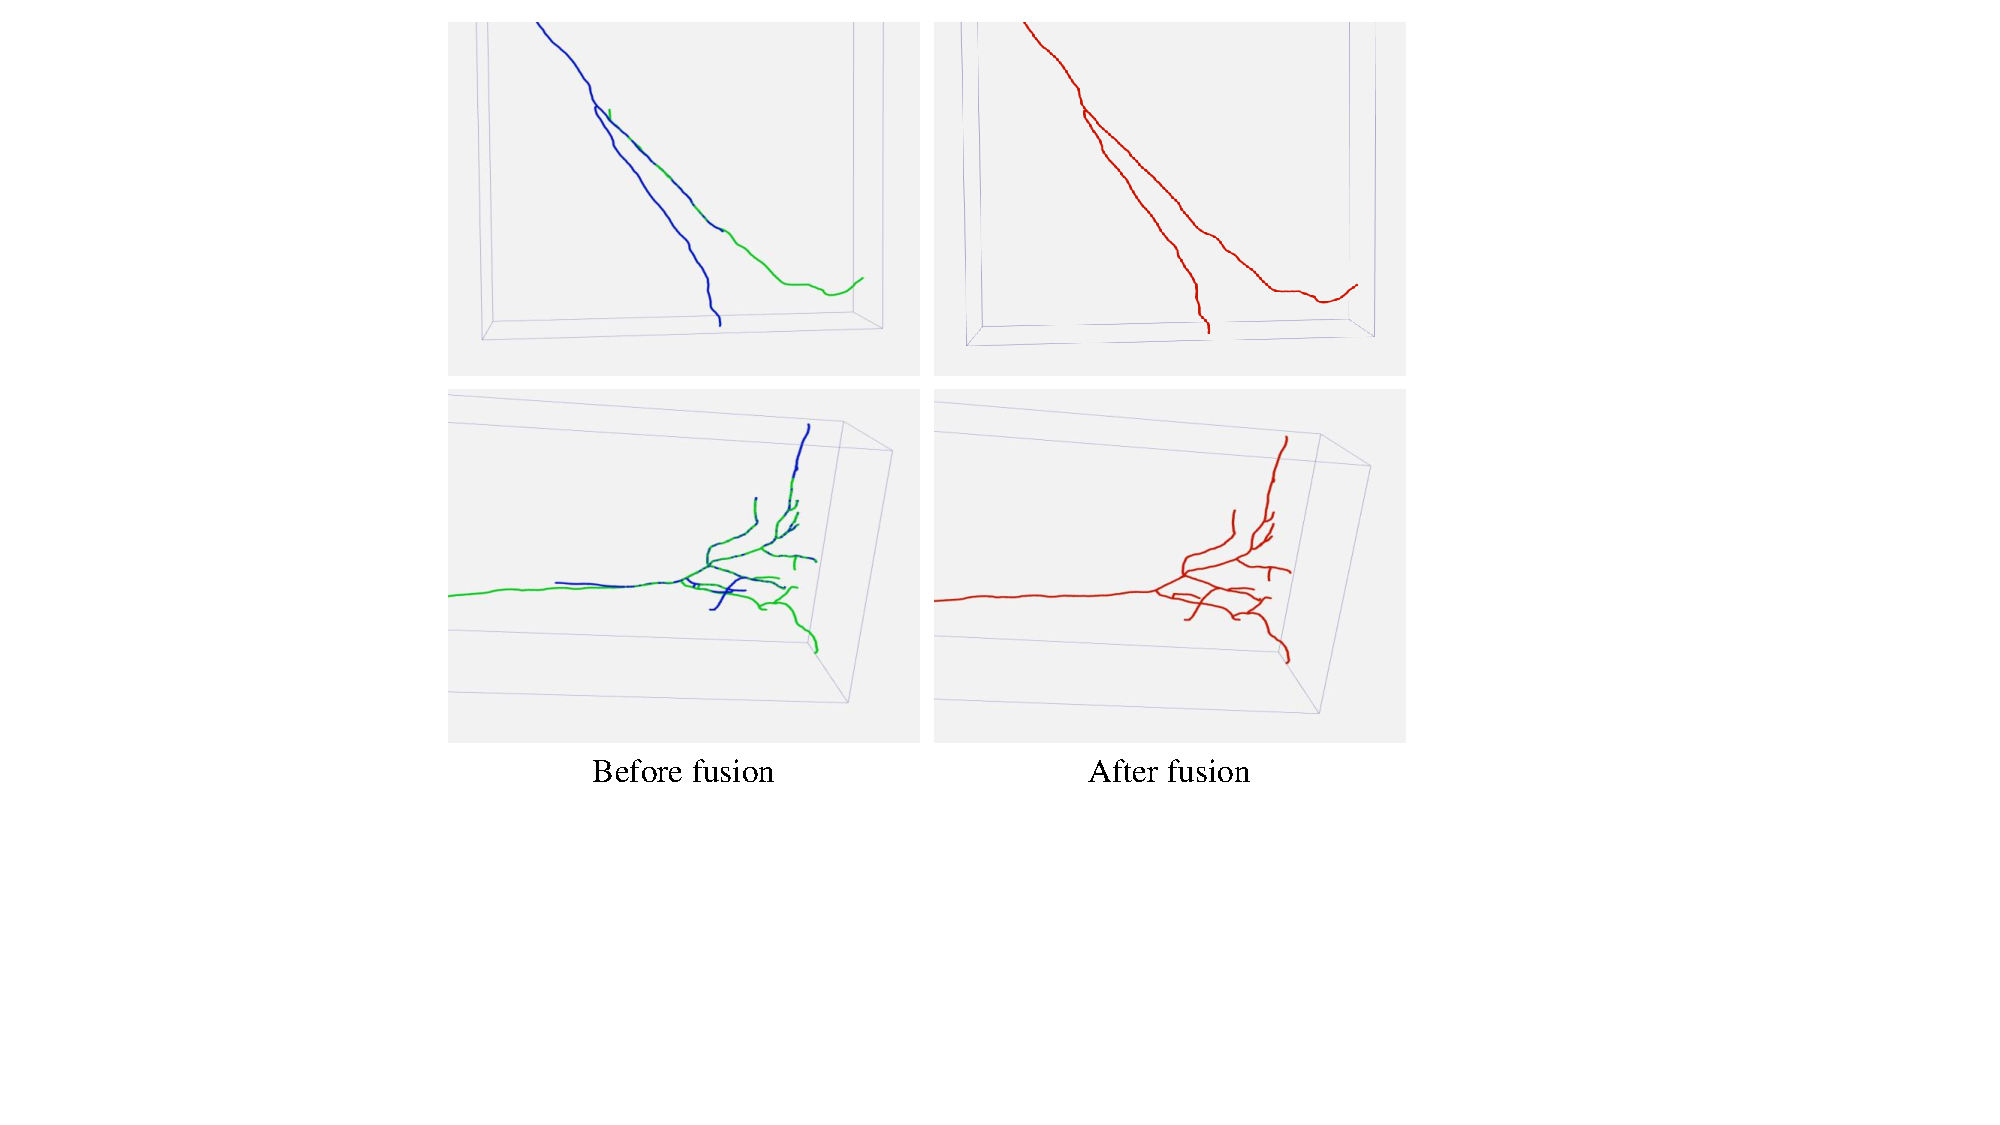
\includegraphics[width=1\columnwidth]{./Illustrations/neuorns_fusion2.pdf}
	\caption{Two examples of correcting the over-tracing and topological discrepancy errors by our fusion algorithm. These reconstructions are shown in skeleton mode for better visualization.}
	\label{fig:overlap_discrepancy}
\end{figure}

\begin{figure}[t]
	\centering
	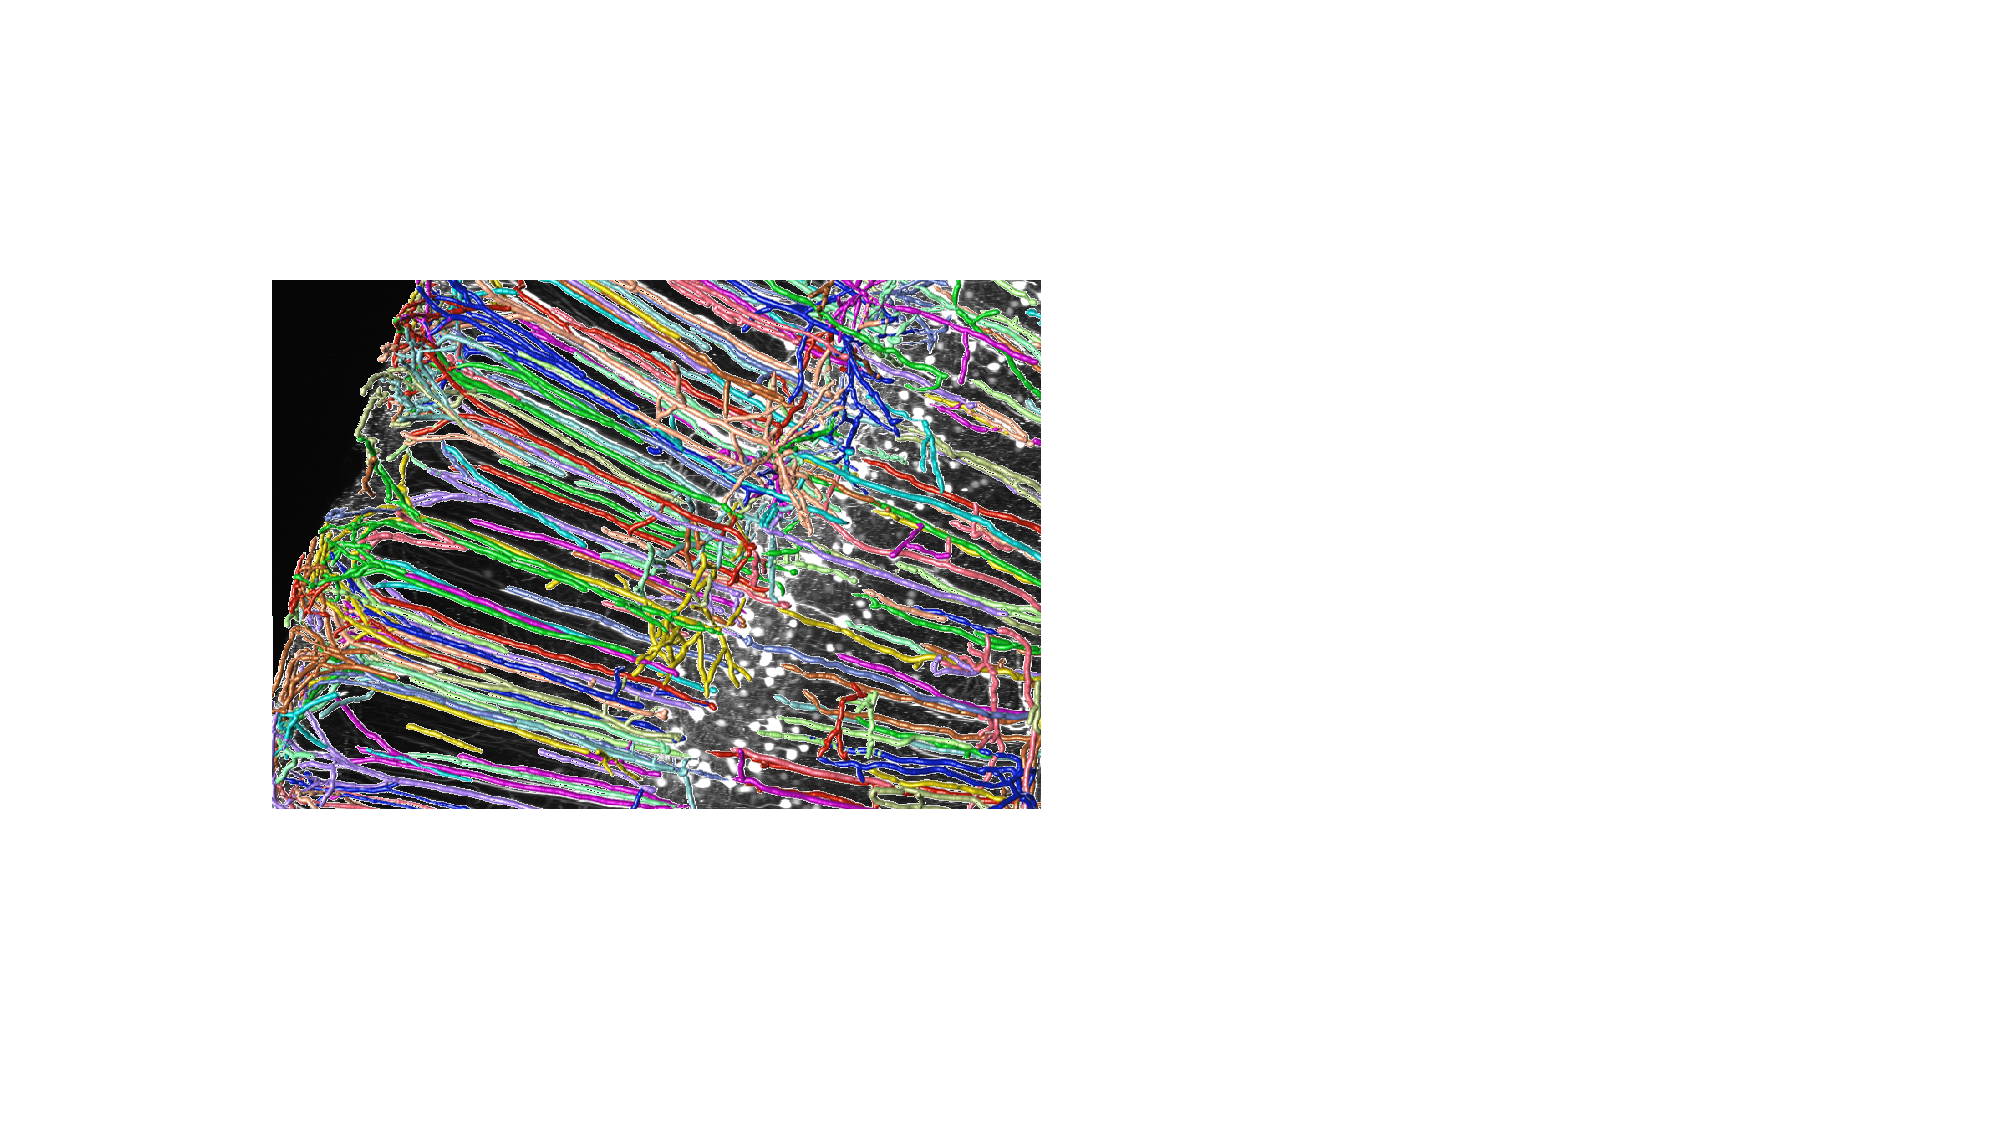
\includegraphics[width=1\columnwidth]{./Illustrations/trace_four_blocks2.pdf}
	\caption{One example of reconstructing neuronal populations from four adjacent blocks using our method. We can observe that, the fragmented neurites from adjacent blocks are assembled continuously and smoothly.}
	\label{fig:reconstruct_blocks}
\end{figure}

Based on the above observations, we design a new fusion algorithm to assemble the matched neurites.
Concretely, we first calculate the length of the two neurites and select the longer one as the reference neurite. Here, we use $\mathcal{N_A}$ to denote the reference neurite, and $\mathcal{N_B}$ to denote another neurite.
Then, for each branch $\mathcal{H_B}$ in neurite $\mathcal{N_B}$, we search in neurite $\mathcal{N_A}$ to see if there is a branch $\mathcal{H_A}$ that overlaps with it.
%
If yes, three steps will be performed to assemble the two branches together.
Firstly, we remove the neuronal compartments in branch $\mathcal{H_A}$ and branch $\mathcal{H_B}$ that near the boundary of the corresponding block, and all branches that are connected to the removed compartments will also be removed. Here, this distance is set to be $70$ voxels.
Secondly, for each neuronal compartment in branch $\mathcal{H_B}$, if there are compartments of branch $\mathcal{H_A}$ around it, it will be removed; otherwise, it is considered to be valid. The searching radius is empirically set to be $10$ voxels.
%Thirdly, by searching the nearest compartment in branch $\mathcal{H_A}$, the modified branch $\mathcal{H_B}$ is connected to $\mathcal{H_A}$.
Thirdly, the first compartment in the modified branch $\mathcal{H_B}$ is connected to $\mathcal{H_A}$ by searching the nearest compartment in branch $\mathcal{H_A}$. 
%In this way, branches in neurite $\mathcal{N_B}$ can be merged with the neurite $\mathcal{N_A}$.
When all branches $\mathcal{H_B}$ overlapping with the neurite $\mathcal{N_A}$ are processed, we can obtain the assembled neurite $\mathcal{N_{AB}}$.
If there are remaining branches $\mathcal{H_B}$ which are not overlapped with neurite $\mathcal{N_A}$, the $\mathcal{N_{AB}}$ will be updated by assembling the remaining branches $\mathcal{H_B}$.
%After all branch $\mathcal{H_B}$ overlapping with neurite $\mathcal{N_A}$ are assembled with neurite $\mathcal{N_A}$, the remaining branches in neurite $\mathcal{N_B}$ will be connected to the assembled neurite $\mathcal{N_{AB}}$ by searching the neatest compartment in $\mathcal{N_{AB}}$.
%In this way, neurite $\mathcal{N_B}$ and neurite $\mathcal{N_A}$ can be merged.



Fig.~\ref{fig:overlap_discrepancy} shows two examples of correcting the over-tracing and topological discrepancy errors by our algorithm.
As shown in Fig.~\ref{fig:reconstruct_blocks}, the neuronal population from four adjacent blocks are successfully reconstructed from the noisy images by our UltraNPR method and the fragment neurites in adjacent blocks are assembled continuously and smoothly.
%It can be seen that the neuronal population is successfully reconstructed from the noisy images and the fragment neurites in adjacent blocks are assembled continuously and smoothly.
%The overall ``UltraNPR"" algorithm can be found in Algorithm~\ref{alg:reconstruction}.


\begin{figure}[t]
	\centering
	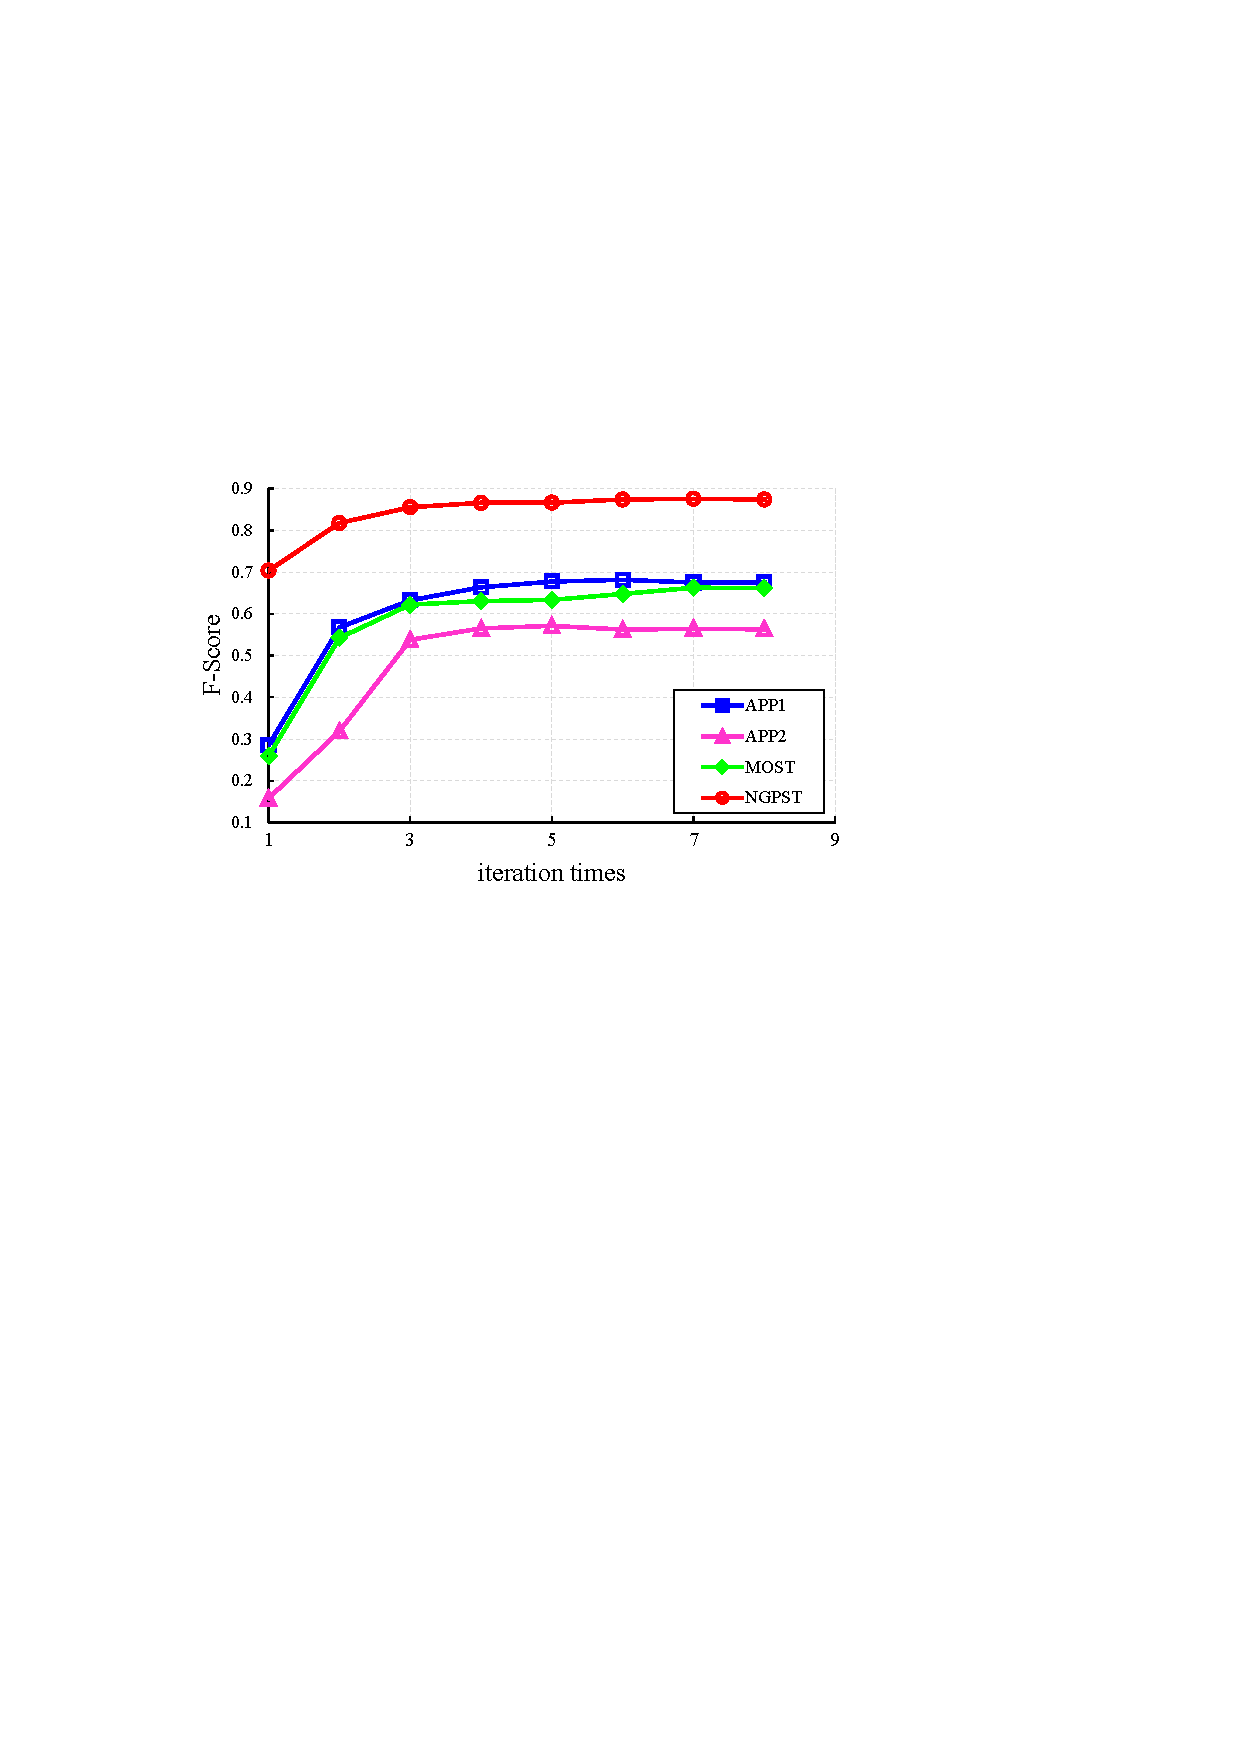
\includegraphics[width=\columnwidth]{./Illustrations/trace_iterations_fscore8.pdf}
	\caption{F-Score of neuron reconstruction using four neuron tracing methods APP1~\cite{Peng2011} and its variant APP2~\cite{Xiao2013}, MOST\cite{Wu2014} and NGPST~\cite{Quan2015} on the VISoR-40 test dataset at eight iterations. For each of the four neuron tracing methods, our approach progressively improves their reconstruction results.} 
	%Plots of other metrics are available in the supplementary materials.}
	\label{fig:fscore_iterations}
\end{figure}

}